\documentclass[12pt]{report}
\usepackage[spanish]{babel}
\usepackage[utf8]{inputenc}
\usepackage{graphicx}
\usepackage{verbatim}
\usepackage{listings}
\usepackage{float}
\renewcommand*\thesection{\arabic{section}}

\begin{document}
	
	\begin{center}
		\textbf{Análisis de Algoritmos, Sem: 2018-1, 3CV1, Práctica 7, 11-2017}
		\newline
	\end{center}
	
	\begin{center}
		\begin{picture}(0,0) \put(-125,-55){
			\includegraphics[width=2.7cm]{../../IPNlogo.jpg}} 
		\end{picture}
		\LARGE Escuela Superior de Cómputo.\\
		Instituto Politécnico Nacional, México.\\
		\begin{picture}(0,0) \put(160,10){
			\includegraphics[width=2.7cm]{../../logoescom.png}} 
		\end{picture}
	\end{center}
	
	\begin{center}
		\Large Práctica 7: Multiplicación de una secuencia de matrices.\\
	\end{center}
	
	\begin{center}
		\textbf{Blancas Pérez Bryan Israel}\\
		orionmunecaycanica@gmail.com\\
	\end{center}
	
	
	\textbf{\large Resumen: }Implementar un algoritmo para encontrar el orden óptimo de multiplicar las matrices de una secuencia de matrices. \newline\\
	\textbf{\large Palabras Clave: } Optimizar, Multiplicación de matrices, Secuencia de matrices, Complejidad Computacional.\\
	


	\section{Introducción}
	En esta práctica se implementará un algoritmo que de como salida, la mejor configuración de paréntesis para efectuar la multiplicación de una secuencia de matrices. Esto es con el fin de no multiplicar la secuencia conforme están ordenadas las matrices, ya que esto puede hacer que se realicen más operaciones escalares entre los elementos de las matrices. En este caso, lo óptimo, es realizar todas las multiplicaciones entre las matrices haciendo el menor número de productos escalares. \newpage
	

	\section{Conceptos Básicos}
	\textbf{Multiplicación de una secuencia de matrices.}\\
		
	Supongamos que tenemos un secuencia de 3 matrices que queremos multiplicar.\\
	
	Sea $A_{10x100} \ B_{100x5} \ y \ C_{5x50}$, y supongamos dos configuración de paréntesis diferentes.\\
	
	Configuración 1.\\
	$(AB)_{10x5} \ -> \ 10x100x5 = 5000$\\
	$(AB)C_{10x50} \ -> \ 10x5x50 = 2500$\\
	Suma total de productos escalares = 7500.\\
	
	Configuración 2.\\
	$(BC)_{100x50} \ -> \ 100x5x50 = 25000$\\
	$A(BC)_{10x50} \ -> \ 10x100x50 = 50000$\\
	Suma total de productos escalares = 75000.\\
	
	Entonces, como se aprecia en el ejemplo anterior, en realidad se puede reducir el número de productos escalares que se realizan, para multiplicar una misma secuencia de matrices, mejorando así, el uso de los recursos del computador. \\En el caso del ejemplo anterior, podemos concluir que multiplicar las matrices con la configuración 1: $((AB)C)$, es mas conveniente que con la configuración 2: $(A(BC))$.\\
	El algoritmo que se implementará más abajo en este reporte, muestra como salida, la mejor configuración de paréntesis de entre todas las posibles.	
	
		
	\newpage
	
	
	\section{Experimentación y Resultados}	
	\textbf{Ejercicio 1.}\\
	Implementar el algoritmo de la multiplicación de una secuencia de matrices.\newline
	i) Como entrada, el algoritmo tendrá $n$ matrices $A_{i}$ de tamaño $P_{i-1}xP_{i}$.\newline
	ii) Como salida, se mostrará la configuración de matrices generada por el algoritmo. \\
	
	
	Pseudocódigo del algoritmo:
	\lstset{language=C, breaklines=true, basicstyle=\footnotesize}
	\lstset{numbers=left, numberstyle=\tiny, stepnumber=1, numbersep=10pt}
	\begin{lstlisting}
secuencia_matrices(P)
  
  n=P.length-1
  M[1,...,n][1,...,n] y S[1,...,n-1][2,...,n]
  
  for i = 1 to n do
    m[i][i] = 0
  
  for l = 2 to n do
    for i = 1 to n-l+1 do
      j = i+l-1
      m[i][j] = infinito
      for k = i to j-1 do
        q = m[i][k] + m[k+1][j] + p[i-1]p[k]p[j]
        if q < m[i][j] then
	      m[i][j] = q
	      s[i][j] = k
	      
  return m y s
  
imprime_parentizacion_optima(s,i,j)
  
  if i = j then
    imprime Ai
  else
    imprime "("
    imprime_parentizacion_optima(s,i,s[i][j])
    imprime_parentizacion_optima(s,s[i][j]+1,j)
    imprime ")"
      
	\end{lstlisting}
	
	Como vemos, el algoritmo hace uso de la función "secuencia de matrices", la cual crea dos matrices que llenará para luego retornarlas. La función " imprime\_parentizacion\_optima", es la que calcula la configuración de paréntesis óptima, y utiliza la matriz s creada en la primer función.\newpage
	
	Resultados.\\
	
	Ejecución 1.
	
	Input.\\
	
		$P=[30,35,15,5]$\\
	
	Output.\\
		
		$(A_{1}(A_{2}A_{3}))$	
	\begin{figure}[H]
		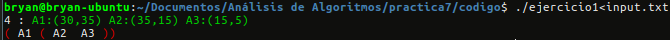
\includegraphics[height=1.5cm,width=16cm]{imagenes/1.png}
		\centering
		\caption{1ra ejecución.}
		\centering
	\end{figure}
	
	Configuraciones posibles para la ejecución 1.\\
	1. $(A_{1}(A_{2}A_{3}))$. Con un total de (30x35x5)+(35x15x5)=7875 operaciones escalares.\\
	2. $((A_{1}A_{2})A_{3})$. Con un total de (30x35x15)+(30x15x5)=18000 operaciones escalares.\\
	
	Por lo tanto concluimos que la salida mostrada por el algoritmo en la figura 1, es en realidad la configuración óptima para multiplicar las matrices.\newpage
	
	Ejecución 2.
	
	Input.\\
	
	$P=[3,5,2,2]$\\
	
	Output.\\
	
	$((A_{1}A_{2})A_{3})$	
	\begin{figure}[H]
		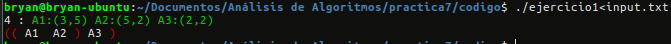
\includegraphics[height=1.5cm,width=16cm]{imagenes/2.png}
		\centering
		\caption{2da ejecución.}
		\centering
	\end{figure}
	
	Configuraciones posibles para la ejecución 2.\\
	1. $(A_{1}(A_{2}A_{3}))$. Con un total de (3x5x2)+(5x2x2)=50 operaciones escalares.\\
	2. $((A_{1}A_{2})A_{3})$. Con un total de (3x5x2)+(3x2x2)=42 operaciones escalares.\\
	
	Por lo tanto concluimos que la salida mostrada por el algoritmo en la figura 1, es en realidad la configuración óptima para multiplicar las matrices.\newpage
	
	
\section{Conclusiones}
Está práctica se me hizo muy sencilla, puesto que los algoritmos eran fáciles de implementar en un lenguaje de programación, pero lo difícil es la lógica implementada. El llenado de las matrices en la función "secuencia\_matrices", es muy complejo de comprender rápido, y me costo entenderle a la perfección. \newline
Tuve algunos problemas al momento de implementar el algoritmo, hasta que decidí hacerlo con matrices de doble apuntador, y memoria dinámica.\newpage 


\section{Anexo}

Problema: Utilizando método por sustitución, muestre:
	\begin{figure}[H]
		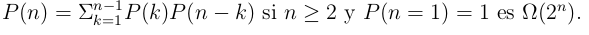
\includegraphics[width=16cm]{imagenes/3.png}
	\end{figure}
	
	Utilizando Sustitución hacia adelante.\\
	$P(n=1)=1$\\
	$P(n=2)=P(1)P(1)=1$\\
	$P(n=3)=P(1)P(2)+P(2)P(1)=2$\\
	$P(n=4)=P(1)P(3)+P(2)P(2)+P(3)P(1)=5$\\
	$P(n=5)=P(1)P(4)+P(2)P(3)+P(3)P(2)+P(4)P(1)=14$\\
	$P(n=6)=P(1)P(5)+P(2)P(4)+P(3)P(3)+P(4)P(2)+P(5)P(1)=42$\\
	
	\begin{table}[htbp]
		\begin{center}
			\begin{tabular}{|l|l|}
				\hline
				\multicolumn{2}{|c|}{Tabla de valores} \\ 
				\hline
				\textbf{n} & \textbf{P(n)}\\
				\hline
				1 & 1 \\ \hline
				2 & 1 \\ \hline
				3 & 5 \\ \hline
				4 & 5 \\ \hline
				5 & 14 \\ \hline
				6 & 42 \\ \hline
				10 & 4862 \\ \hline
				15 & 2674440 \\ \hline
				
			\end{tabular}
			\caption{Tabla de valores de P(n).}
			\label{tabla:analisis1}
		\end{center}
	\end{table}

Por lo tanto vemos que la función tiene un comportamiento exponencial.\\
 
	$Por \ lo \ tanto \ P(n)  \epsilon \ \Omega (2^{n}).$\\
	\newpage

\section{Bibliografía}

https://es.wikibooks.org/wiki/Optimizaci\%C3\%B3n\_del\_Producto\_de\_Matrices
	
\end{document}